% questions.tex —— 1977 年·江苏苏州市初试卷 · 题目内容片段（无答案）
% 由 tools/generate_projects.py 依来源总账自 1977/1977_数学真题_江苏苏州市初试_试题.md 生成，勿手改（改源 MD 后重跑）


\gkpart{江苏苏州市初试卷}

\begin{gktip}
\textbf{来源说明}：本卷为 1977 年高校招生苏州市初试（预选）数学试卷，依据固定源 PDF 第 1—3 页逐题转录。源 PDF 为汇编材料扫描件，第 1 页页首印有分节标题「四、苏州市」（H1 按原卷逐字转写），第 2 页左下角印有原书页码 236，第 1、3 页无页码。原卷大题号用中文数字「一、……六、」，本库转写为「\textbf{N．}」；大题一标注「（每小题 5 分）」，内含 12 个小题，原卷用阿拉伯数字「1．2．…12．」编号，本库统一转写为「（N）」。大题二、四、五、六标有分值，大题三原卷未见分值标注，如实转录不补写。原卷末尾另有「附加题」两题（各 10 分），源卷自成编号「1.」「2.」，不计入正式题量。源卷为纯题面扫描，未附答案；配套答案与解析为本库编者独立推导，\textbf{非官方标准答案}。
\end{gktip}

\par\medskip

\Needspace{0.4\textheight}
\begin{question}
\gkti{1}\textbf{（每小题 5 分）} 

\Needspace{5\baselineskip}
（1） 计算：

\nopagebreak[4]
\[
1\div\left(-\frac18\right)^2\times\left(-\frac14\right)^3+\left(-1\frac13\right)^2\div\left(\frac23\right)^2.
\]

（2） 已知：$3:x=6:y$，求 $\dfrac{x}{y}=?$

（3） 若 $\sqrt{(3-x)^2}=x-3$ 成立，求 $x$ 的取值范围。

（4） 求函数 $y=\dfrac{1}{2x^2-5x-3}$ 的自变量 $x$ 的取值范围。

（5） 若 $0.0054=5.4\times10^n$，求 $n$。

（6） 解方程：$(2x-3)(x+4)=-5$。

（7） 求 $\sin(-1020^\circ)$ 的值。

（8） 已知 $\lg2=0.3010$，$\lg3=0.4771$，求 $\lg1800$ 的值。

\Needspace{5\baselineskip}
（9） 求

\nopagebreak[4]
\[
\lim_{n\to\infty}\frac{2n+1}{n}
\]

的值。

（10） 求过点 $(3,4)$ 并平行于直线 $2x+y-5=0$ 的直线方程。

（11） 极坐标方程 $\rho=3$ 表示什么曲线；并且将它化成直角坐标方程。

（12） 某种反射镜面是旋转抛物面，它的镜面口直径是 $40$ 厘米，深度是 $5$ 厘米（如图），求抛物线的直角坐标方程和焦点坐标。
\nopagebreak[4]
\begin{center}% 1977 年江苏苏州市初试卷第 1 题第 (12) 小题：旋转抛物面反射镜面轴向剖面示意图，
% 顶点 O 在原点，对称轴沿 X 轴、开口向右；虚线分别标示镜口半径方向（40）与轴向深度（5）（按源卷第 2 页布局重绘，非原图比例）
\begin{tikzpicture}[scale=1,>=stealth]
  \draw[->] (-0.6,0) -- (3.0,0) node[right] {$X$};
  \draw[->] (0,-2.0) -- (0,2.2) node[above] {$Y$};
  \node[below left] at (0,0) {$O$};
  \draw[thick] (0,0) .. controls (0.6,0.9) and (1.4,1.4) .. (2.0,1.5);
  \draw[thick] (0,0) .. controls (0.6,-0.9) and (1.4,-1.4) .. (2.0,-1.5);
  \draw[dashed] (2.0,1.5) -- (2.0,-1.5);
  \node[right] at (2.05,0) {$40$};
  \draw[dashed] (0,-1.8) -- (2.0,-1.8);
  \node[below] at (1.0,-1.85) {$5$};
\end{tikzpicture}
\end{center}
\nopagebreak[4]
\end{question}
\begin{question}
\gkti{2}\textbf{（8 分）} 化简：

\nopagebreak[4]
\[
\left[a^{-\frac32}b\left(ab^{-2}\right)^{-\frac12}\right]^3,
\]

并求当 $a=\dfrac{1}{\sqrt2}$，$b=\dfrac{1}{\sqrt[3]2}$ 时的值。

\end{question}
\begin{question}
\gkti{3}已知 $\cos\theta=0.6$，并且 $\theta$ 是第四象限的角，求 $\sin2\theta$ 的值。

\end{question}
\begin{question}
\gkti{4}\textbf{（8 分）} 将 $40$ 分成两个正数，使它们的平方和为最小，求这两个数。

\end{question}
\begin{question}
\gkti{5}\textbf{（8 分）} 已知 $A\text{、}B$ 两地相距 $600$ 公里，从 $A$ 地开往 $B$ 地的客车每小时比货车快 $15$ 公里，客车比货车少用 $2$ 小时，求客车和货车的速度。

\Needspace{0.4\textheight}
\end{question}
\begin{question}
\gkti{6}\textbf{（8 分）} $MT$ 是 $\odot O$ 的切线，$O$ 是圆心，$T$ 是切点，$MO$ 与 $\odot O$ 交于 $A$ 点，已知 $MA$ 的长为 $h$，$\odot O$ 的半径为 $r$，$TP$ 为 $MO$ 的垂线，垂足是 $P$，求 $TP$ 的长。
\nopagebreak[4]
\begin{center}% 1977 年江苏苏州市初试卷第 6 题：MT 是 ⊙O 的切线，T 为切点，
% O、P、A、M 依次在同一直线上，TP⊥MO 交于 P（按源卷第 3 页布局）
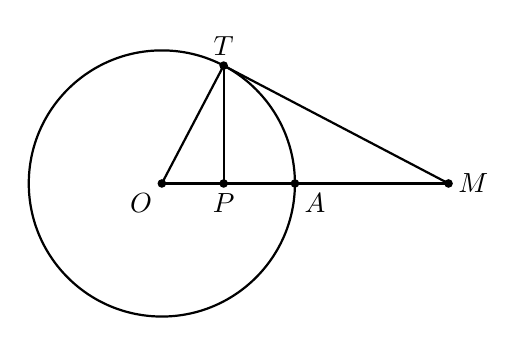
\begin{tikzpicture}[scale=1.3]
  \coordinate (O) at (0,0);
  \coordinate (M) at (2.8,0);
  \coordinate (A) at (1.3,0);
  \coordinate (P) at (0.6036,0);
  \coordinate (T) at (0.6036,1.1514);
  \draw[thick] (O) circle (1.3);
  \draw[thick] (O) -- (M);
  \draw[thick] (O) -- (T);
  \draw[thick] (T) -- (M);
  \draw[thick] (T) -- (P);
  \fill (O) circle (1.2pt) node[below left] {$O$};
  \fill (P) circle (1.2pt) node[below] {$P$};
  \fill (A) circle (1.2pt) node[below right] {$A$};
  \fill (M) circle (1.2pt) node[right] {$M$};
  \fill (T) circle (1.2pt) node[above] {$T$};
\end{tikzpicture}
\end{center}
\nopagebreak[4]
\textbf{附加题 1．（10 分）} 如果二次方程 $(m+1)x^2+(2m-1)x+(m-1)=0$ 无实数根，求证：二次方程 $(m-3)x^2-2(m+3)x-(m+5)=0$ 一定有两个不相等的实根。

\textbf{附加题 2．（10 分）} $\triangle ABC$ 的面积为 $10\sqrt3$，周长为 $20$，并且三个内角成等差数列，求各边的长。

\end{question}